\documentclass{beamer}
\usepackage{hyperref}
\hypersetup{unicode=true}
\usepackage[utf8x]{inputenc}
\usepackage[english,russian]{babel}
\usepackage{beamerthemesplit}
\graphicspath{{pics/}}



% блок для добавления значка зергов
\usepackage[absolute,verbose,overlay]{textpos}
\newcommand{\zerglogo}{% 
  \setlength{\TPHorizModule}{11.8 cm} 
  \setlength{\TPVertModule}{1.1 cm} 
  \begin{textblock}{1}(1,1) 
   
\includegraphics[height = 9 mm]{zerg.png} 
  \end{textblock}}


\usepackage{color}
\definecolor{gray}{rgb}{0.4,0.4,0.4}
\definecolor{bggray}{rgb}{0.9,0.9,0.9}
%	Параметры подсветки исходного кода на C++
\usepackage{listings}
\lstset{breakatwhitespace,
	language=C++,
	columns=fullflexible,
	keepspaces,
	breaklines,
	tabsize=3,
	numbers=left, % нумерация строк
	numberstyle=\small\color{gray},
	numbersep=5pt,
	backgroundcolor=\color{bggray},
	showstringspaces=false,
	extendedchars=true,
	keywordstyle=\color{blue}\ttfamily,
	stringstyle=\color{red}\ttfamily,
	commentstyle=\color{green}\ttfamily,
	morecomment=[l][\color{magenta}]{\#}
}


\begin{document}
\title[Численные методы акустооптики на C++]{Отчёт о ведении спецкурса \\"Численные методы в приложении к задачам акустооптики и акустоэлектроники на языке программирования С++" в 2012 году}
\author{Арсений Трушин \& \(Co\)} 
\date{\today}

%% %	Пример листинга на C++, отступы, включая отступы от начала строки сохраняются (!)
%% \defverbatim[colored]\lst{
%%   \begin{lstlisting}[tabsize=2,basicstyle=\ttfamily]
%%     const char *processing() const{
%%       somestring = "-1";
%%     }
%% \end{lstlisting}}

%% %	Вставка листинга на C++
%% \frametitle{Пример кода на C++}
%% \lst

%	Слайд-заголовок (#1)
\frame{\titlepage}
%	Слайд с содержанием презентации (#2)
\frame{\frametitle{Содержание}\tableofcontents} 

\section{Обзор. Цели и методы спецкурса.}
\subsection{Проблема}
\frame{
  \frametitle{Преподавание программирования на Физфаке}
  \begin{block}{Первые курсы}
    \begin{itemize}
    \item На первых курсах есть C++
    \item Рассказывают о Win32API
    \item Не рассказывают о STL
    \end{itemize}
  \end{block}
  \begin{block}{В рамках спецкурса}
    \begin{itemize}
    \item Решение практических задач
    \item ``Точки входа'' в полезные технологии
    \item Решения в ``две строчки''
    \end{itemize}
  \end{block}
}
%
\subsection{Предлагаемое решение}
\frame{
  \frametitle{Особенности спецкурса}
  \begin{block}{Организационные}
    \begin{itemize}
    \item Маленькая группа - адаптивность
    \item Нацеленность на актуальные задачи
    \end{itemize}
  \end{block}
%
  \begin{block}{Технологии}
    \begin{itemize}
      \item g++/mingw
      \item emacs
      \item git
      \item povray
    \end{itemize}
  \end{block}
}
%
\section{Рассмотренные задачи и инструменты}
\subsection{Подбор констант для кристалла ниобата лития}
\subsubsection{Уравнения Кристоффеля для ниобата лития}

\begin{frame}{Уравнения эластодинамики для пьезоэлектрика}
	
\begin{columns}
\column{7 cm}
	\begin{block}{Уравнения Кристоффеля:}

\ $\Gamma_{il} p_l = \rho V^2 p_i$\\

\ $\Gamma_{il} = \bar{c}_{ijkl} n_j n_k$ -- компоненты тензора Кристоффеля

\ $\lambda=\rho V^2$

  \end{block}
	
  \begin{block}{Пьезоэффект:}
	
\ $\bar{c}_{ijkl} = c_{ijkl}^E + (e_{pij} n_{p}) (e_{qhl} n_{q}) / \varepsilon_{jk}^S n_{j} n_{k}$

\ $e_{pij}, e_{qhl}$ -- пьезоэлектрические модули

\ $\varepsilon_{jk}^S$ -- диэлектрическая проницаемость

  \end{block}
	
\column{5 cm}
	
\begin{figure}

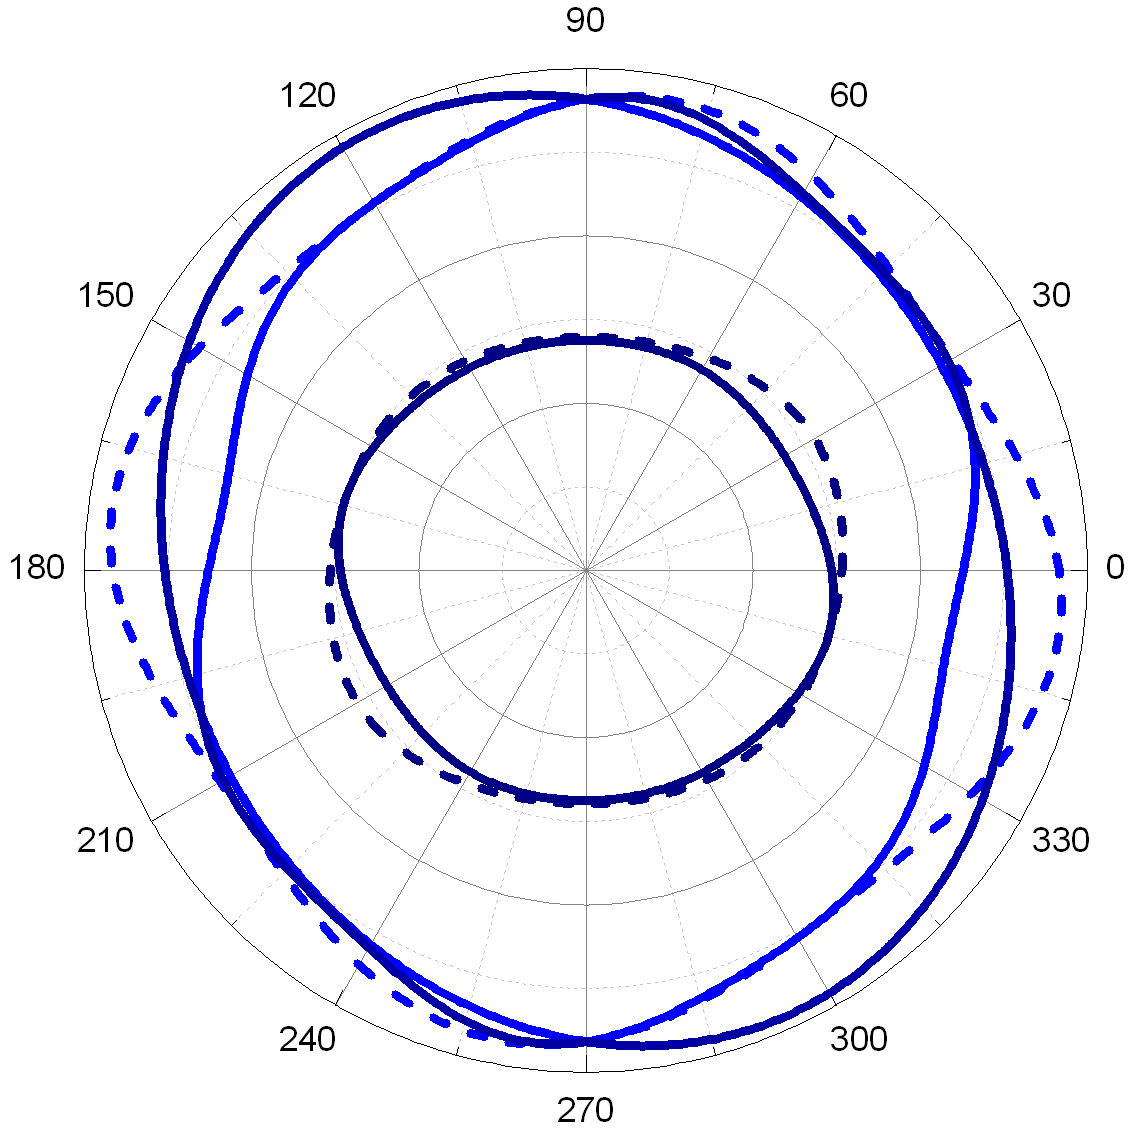
\includegraphics[width=5 cm]{linbo3_piezo.png}

\end{figure}

\end{columns}
\end{frame}

%
\subsubsection{Экстракция экспериментальных данных}
\frame{
   \frametitle{Проблемы извлечения данных}
   \begin{columns}
     \column{6 cm}
     \begin{figure}
       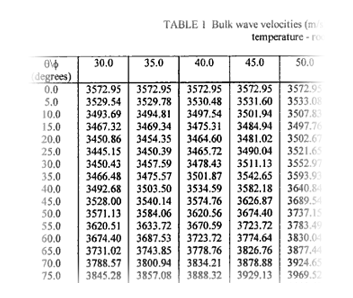
\includegraphics[width = 6cm]{table_example.png}
     \end{figure}
     \column{7 cm}
     \begin{table}
       \begin{tabular}{ c  c  c  c }
         \hline 
         $\theta \backslash \varphi$ & 30.0 & 35.0 & 40.0 \\
         \hline
         0.0  & 3572.95 & 3572.95 & 3572.95 \\
         5.0  & 3529.54 & 3529.78 & 3530.48 \\
         10.0 & 3493.69 & 3494.81 & 3497.54 \\
         15.0 & 3467.32 & 3469.34 & 3475.31 \\
         \hline
       \end{tabular}
     \end{table}
   \end{columns}

    
{\scriptsize 
\vspace*{\baselineskip}
[1] K.K. Wong, Properties of Lithium Niobate, INSPEC, London, 2002}
\vspace*{\baselineskip}
}
\frame{
  \frametitle{Проблемы извлечения данных}
   \begin{block}{Шаги подготовки данных}
    \begin{itemize}
      \item Перевод данных из графического в тестовый вид \\ {\hspace{6 cm} \footnotesize{OCR программы}}

      \item Считывание данных из txt в основную программу

      \item Устранение ошибок распознавания \\ {\hspace{6 cm} \footnotesize{B542,\% $\rightarrow$ 8542.96}}

      \item Поиск численных ошибок по величине невязки \\ {\hspace{6 cm} \footnotesize{8542.96 $\rightarrow$ 3542.96}}
    \end{itemize}
  \end{block}
}

%
\subsubsection{Метод отжига}
\frame{
  \frametitle{Метод отжига}
  \begin{block}{Начальные условия}
    \begin{itemize}
      \item Начальный набор констант $\{c^0_{ijkl}\}, \{e^0_{pij}\}, \{\epsilon^0_{jk}\}$ из Кушибики
      \item Экспериментальные значения скоростей $V_i(\phi, \theta)$ Книжка 
    \end{itemize}
  \end{block}
  \begin{block}{Хотим}
    \begin{itemize}
      \item Получить набор констант $\{c_{ijkl}\}, \{e_{pij}\}, \{\epsilon_{jk}\}$ дающий скорости максимально близкие к экспериментальным
    \end{itemize}
  \end{block}
}
\frame{
  \frametitle{Метод отжига}
  \begin{columns}
    \column{7 cm}
      \begin{itemize}
      \item Случайно выбираем параметр из $\{c^0_{ijkl}\}, \{e^0_{pij}\}, \{\epsilon^0_{jk}\}$, изменяем его на $\delta(T)$, расчитываем текущие скорости
      \item Считаем невязку текущих и экспериментальных скоростей $\Delta^{curr}$
      \item Если $\exp(-\frac{\Delta^{curr}-\Delta^{best}}{T}) > rand[0,1] \Rightarrow$ запоминаем текущие параметры как лучшие
%$\Delta^{curr} \rightarrow \Delta^{best}$; $V^{curr} \rightarrow V^$
      \item Повторяем пока не получим желаемый $\Delta^{best}$
      \end{itemize}
    \column{5 cm}
    \begin{figure}
      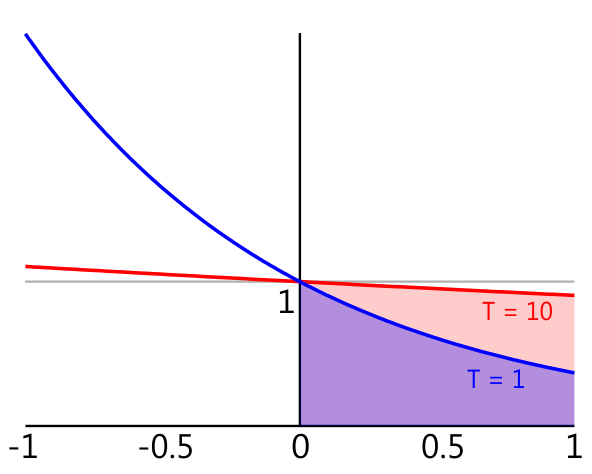
\includegraphics[width = 5cm]{exponent.png}
    \end{figure}
  \end{columns}

}
%
\subsubsection{Рой}
\frame{
  \frametitle{Рой}
  \zerglogo

  Никита
}

{
\frame{
  \frametitle{Сравнение результатов}
  \scriptsize 
  \begin{table}
    \centering
    \begin{tabular}{l c c c c c c c}
      \multicolumn{8}{c}{Константы упругости, [$\times 10^{10}$ Н/м$^2$]} \\
      \hline
      & $c_{11}$ & $c_{12}$ & $c_{13}$ & $c_{14}$ & $c_{33}$ & $c_{44}$ & $c_{66}$ \\
      \hline
      Ворнер [2] & 20,3$~~~$ & 5,3$~~~$ & 7,5$~~~$ & 0,9$~~~$ & 24,5$~~~$ & 6,0$~~~$ & 7,5$~~~$ \\
      Кушибики [3]  & 19,886 & 5,467 & 6,799 & 0,783 & 23,418 & 5,985 & 7,209 \\
      Кондратьев & --- & --- & --- & --- & --- & --- & --- \\
      Терехов  & 20,377 & 5,774 & 7,535 & 0,852 & 24,314 & 5,980 & 7,308 \\
      Трушин & 20,381 & 5,764 & 7,547 & 0,854 & 24,324 & 5,978 & 7,309 \\
      \hline
    \end{tabular}
  \end{table}
  \begin{columns}
    \column{7cm}
    \begin{table}
      \begin{tabular}{l c c c c}
        \multicolumn{5}{c}{Пьезоэлектрические константы, [Кл/м$^2$]} \\
        \hline 
        & $e_{15}$ & $e_{22}$ & $e_{31}$ & $e_{33}$  \\
        \hline
        Ворнер [2] & 3,7$~~~$ & 2,5$~~~$ & 0,2$~~~$ & 1,3$~~~$ \\
        Кушибики [3] & 3,655 & 2,407 & 0,328 & 1,874  \\
        Кондратьев & --- & --- & --- & --- \\
        Терехов  & 3,900 & 2,529 & 0,252 & 1,378  \\
        Трушин & 3,954 & 2,560 & 0,242 & 1,373  \\
        \hline
      \end{tabular}
    \end{table}
    \column{5cm}
    \begin{table}
      \begin{tabular}{l c c}
        \multicolumn{3}{c}{Диэлектрические константы} \\
        \hline 
        & $\varepsilon_{11}/\varepsilon_{0}$ & $\varepsilon_{33}/\varepsilon_{0}$  \\
        \hline
        Ворнер [2] & 44$~~$ & 29$~~$  \\
        Кушибики [3] & 44,9 & 26,7   \\
        Кондратьев & --- & --- \\
        Терехов  & 47,7 & 30,2   \\
        Трушин & 48,9 & 30,6   \\
        \hline
      \end{tabular}
    \end{table}
  \end{columns}

    [2] A.W. Warner {\it{et al.}, J. Acoust. Soc. Amer.}, \textbf{42}, 1967
            
    \vspace*{-0.1cm}
    [3] J. Kushibiki {\it{et al.}, IEEE Trans. Ultrason., Ferroelect., Freq. Contr.}, \textbf{41}, 1994
    \vspace*{\baselineskip}
}
}
%  cfmat[0] = 19.886;
%  cfmat[1] = 5.467;
%  cfmat[2] = 6.799;
%  cfmat[3] = 0.783;
%  cfmat[4] = 23.418;
%  cfmat[5] = 5.985;
%  cfmat[6] = 7.209;

%  cfpiezo[0] = 3.655;
%  cfpiezo[1] = 2.407;
%  cfpiezo[2] = 0.328;
%  cfpiezo[3] = 1.894;

%  cfeps[0] = 44.9;
%  cfeps[1] = 26.7;

%c11(2.0381e+11), c12(5.76401e+10), c13(7.54693e+10), 
%c14(8.54231e+09), c33(2.43238e+11), c44(5.97824e+10), 
%c66(7.30857e+10), e15(3.9536), e22(2.5595), 
%e31(0.241836), e33(1.37299), exxc(48.9306), ezzc(30.6026)

%cfmat[0] = 20.3772; cfmat[1] = 5.77351; cfmat[2] = 7.53455;
%cfmat[3] = 0.852367; cfmat[4] = 24.314; cfmat[5] = 5.98046;
%cfmat[6] = 7.30832; cfpiezo[0] = 3.90042; cfpiezo[1] = 2.52895;
%cfpiezo[2] = 0.251757; cfpiezo[3] = 1.37793; cfeps[0] = 47.6565; cfeps[1] = 30.2265;


\subsection{PovRay}
\begin{frame}[fragile]
\frametitle{Пример кода}

\begin{columns}
	\begin{column}{8cm}
	\begin{verbatim}
		background {color <1,1,1>}
		camera {
		location <3,3,3>
		look_at <0,0,0>
		angle 35}

		light_source {<10,10,10> color <1,1,1>}
		light_source {<5,10,5> color <1,1,1>}
		
		sphere {<0,0,0>, 1 pigment {color <0.8,0.3,0.7>}}
		cylinder {<1,0,0>,<1,0,0.5>, 0.15  pigment {color <0,0,1>}}     
		box {<0,-0.3,0.8>, < 0.4,0.1,1.2> pigment {color <0.7,0.6,0.5>}} 

	\end{verbatim}
	\end{column}
	\begin{column}{4.5cm}
		\raisebox{80pt}{
		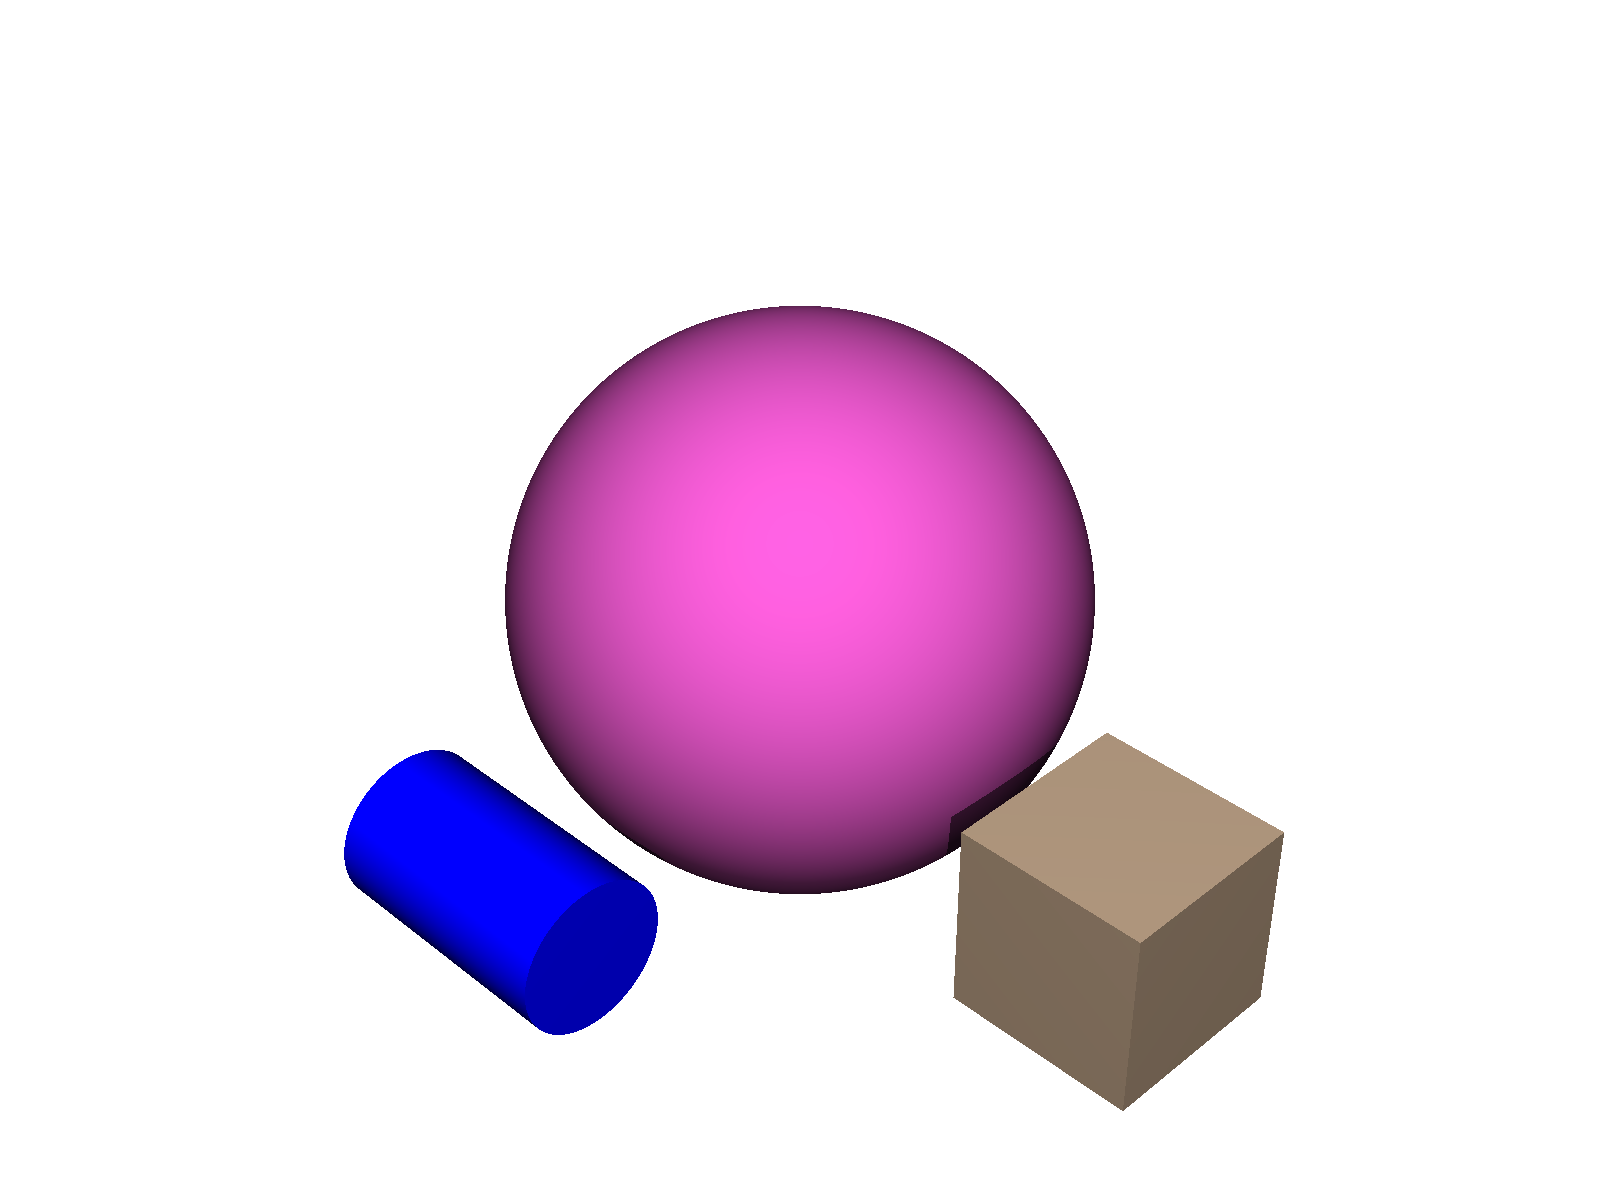
\includegraphics[width=5 cm]{moon_2.png}}
	\end{column}
\end{columns}
	
  %Уже говорилось, что PovRay - это удобный инструмент для визуализиции результатов расчёта, кроме того, он позволяет делать трёхмерные иллюстрации и мультфильмы.
  
\end{frame}

\begin{frame}[fragile]
\frametitle{Наложение текстур}
\begin{verbatim}
#include "textures.inc"
sphere { <0,0,0>, 1 
			  pigment {color <0.8,0.3,0>} texture{name_texture}}
\end{verbatim}
\begin{columns}
	\begin{column}{4cm}	
		
\includegraphics[width=4 cm]{moon_candy.png}
		\centering
		\\Candy\_Cane
	\end{column}
	\begin{column}{4cm}	
		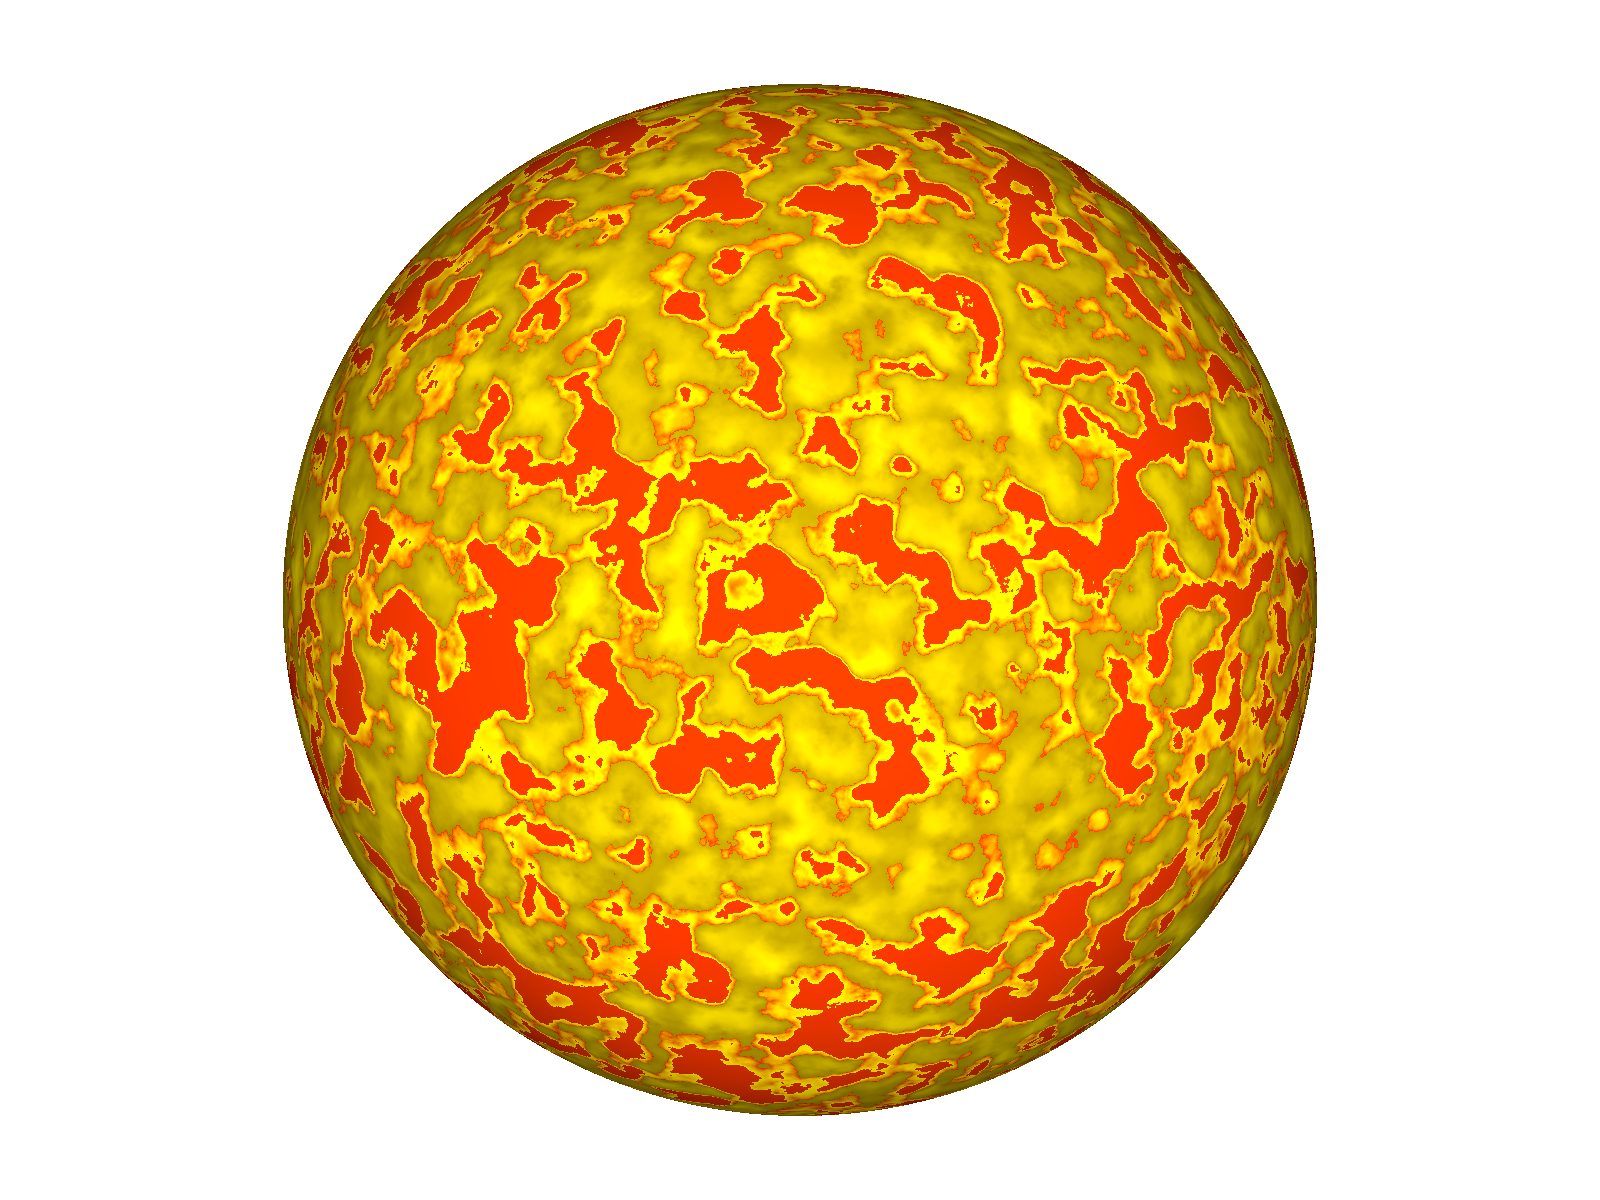
\includegraphics[width=4 cm]{moon_Blood_Sky.png}
		\centering
		\\Blood\_Sky
	\end{column}
	\begin{column}{4cm}	
		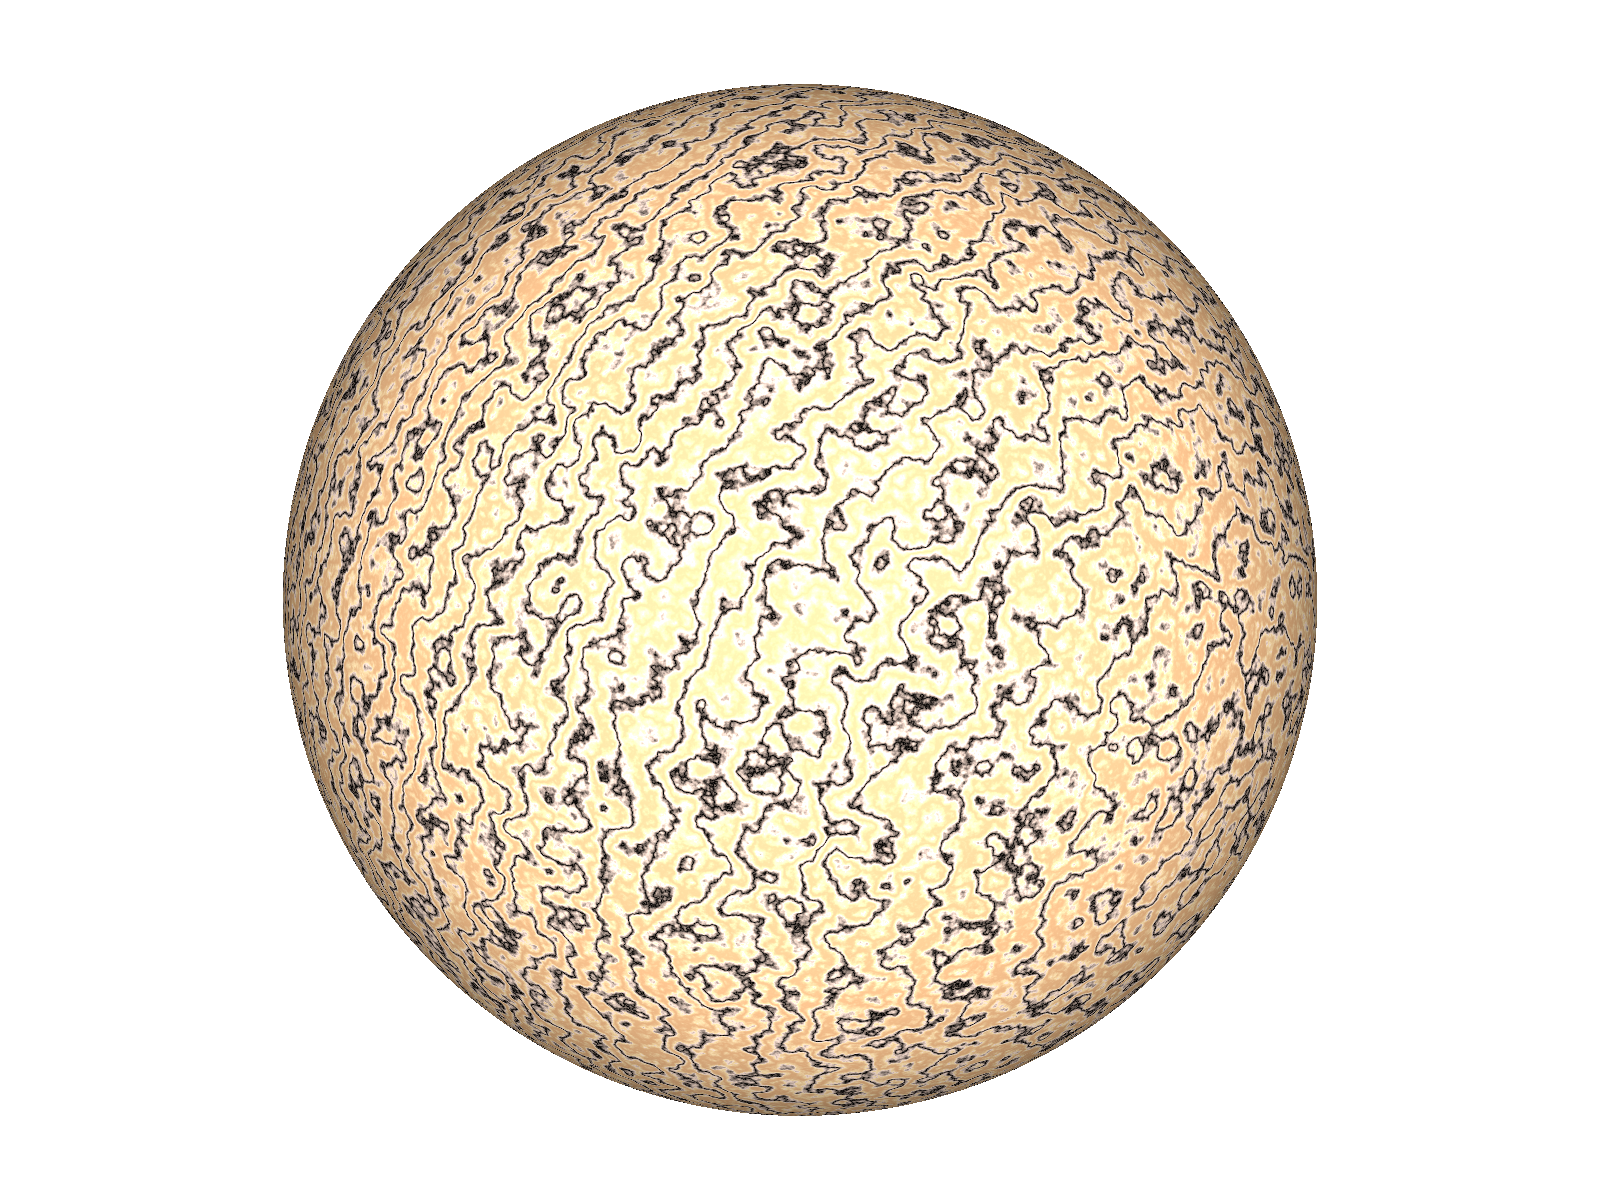
\includegraphics[width=4 cm]{moon_Brown_Agate.png}
		\centering
		\\Brown\_Agate
	\end{column}
\end{columns}
\end{frame}

{\setbeamercolor{background canvas}{bg=black}
\frame{
\frametitle{Луна}
	\begin{center}
		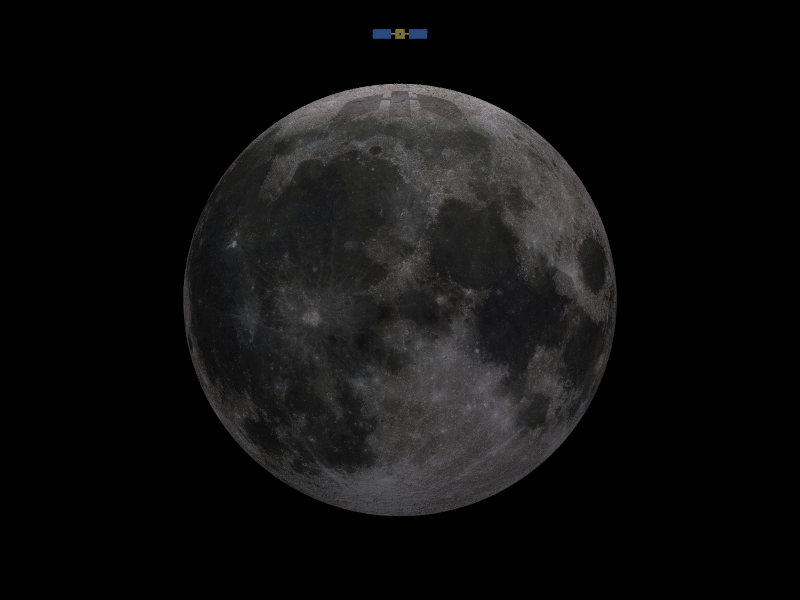
\includegraphics[width=9 cm]{real_moon.png}
	\end{center}
}
}

\frame{ 
  \frametitle{Использование PovRay для визуализации результатов расчёта}

\begin{columns}
	\begin{column}{4cm}	
		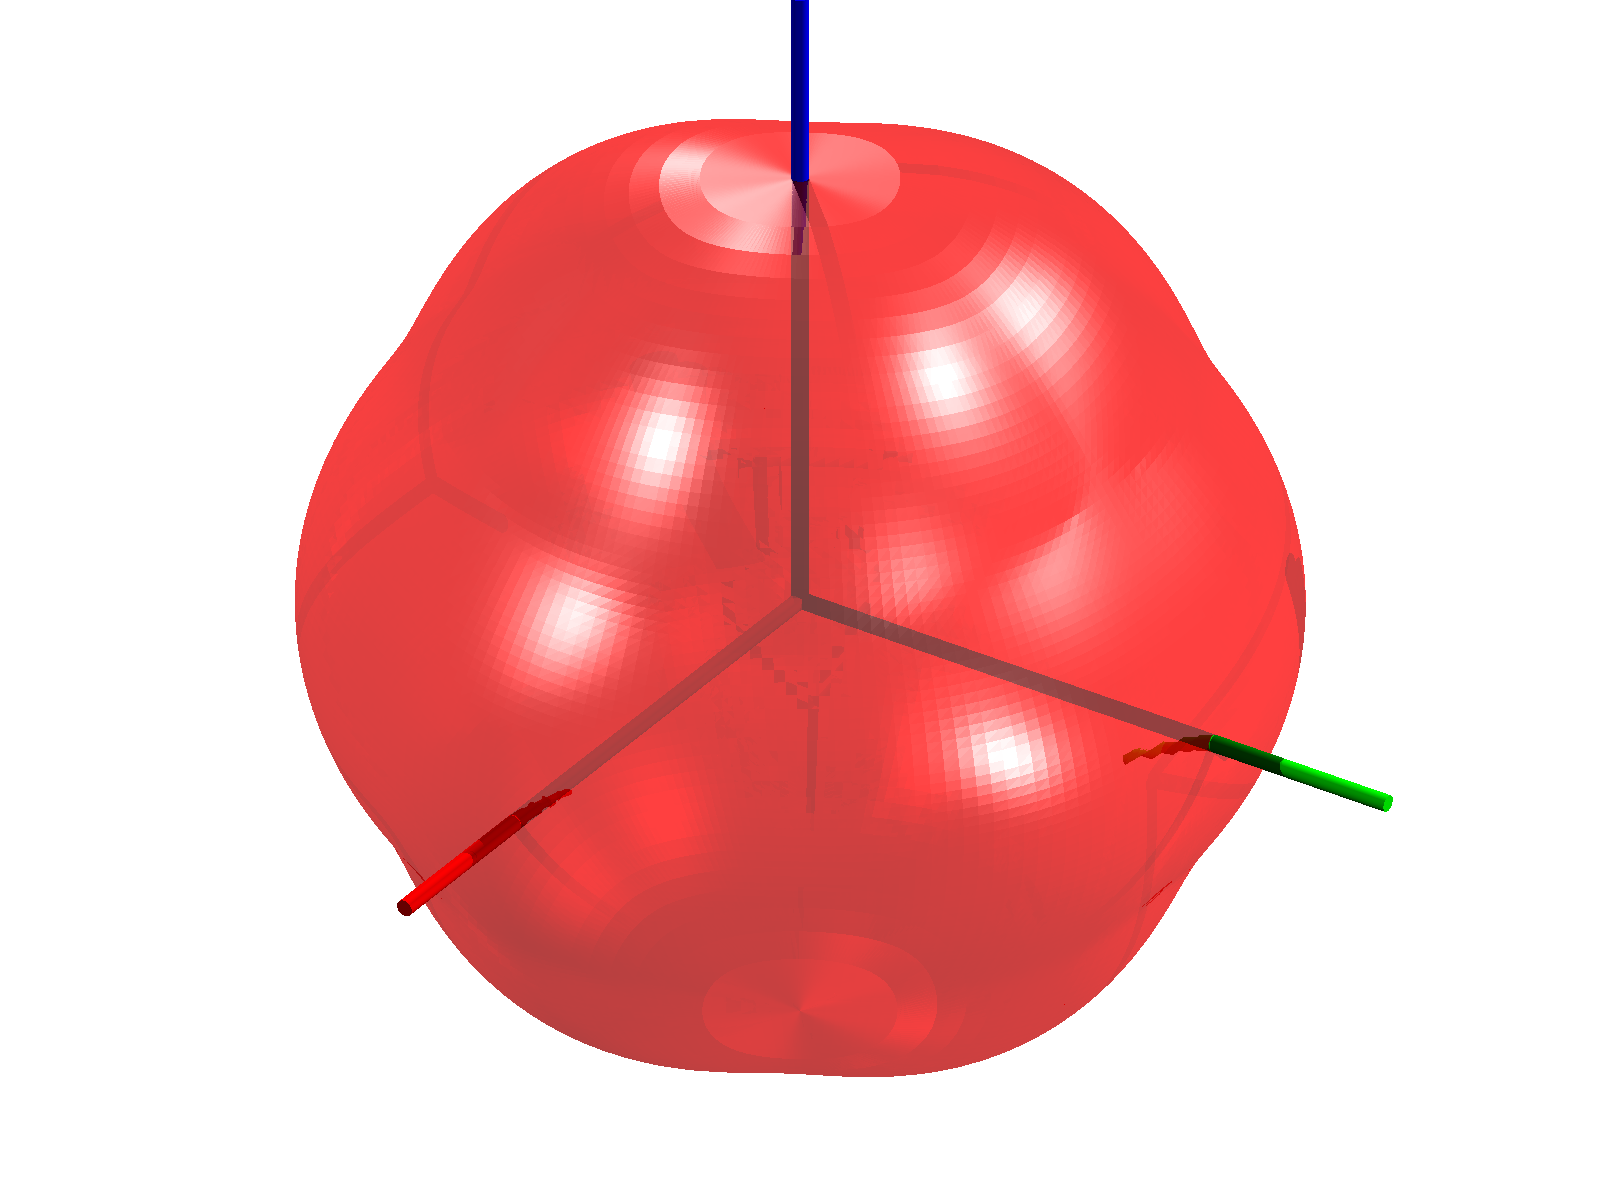
\includegraphics[width=4 cm]{slow_linbo3_0.png}
	\end{column}
	\begin{column}{4cm}	
		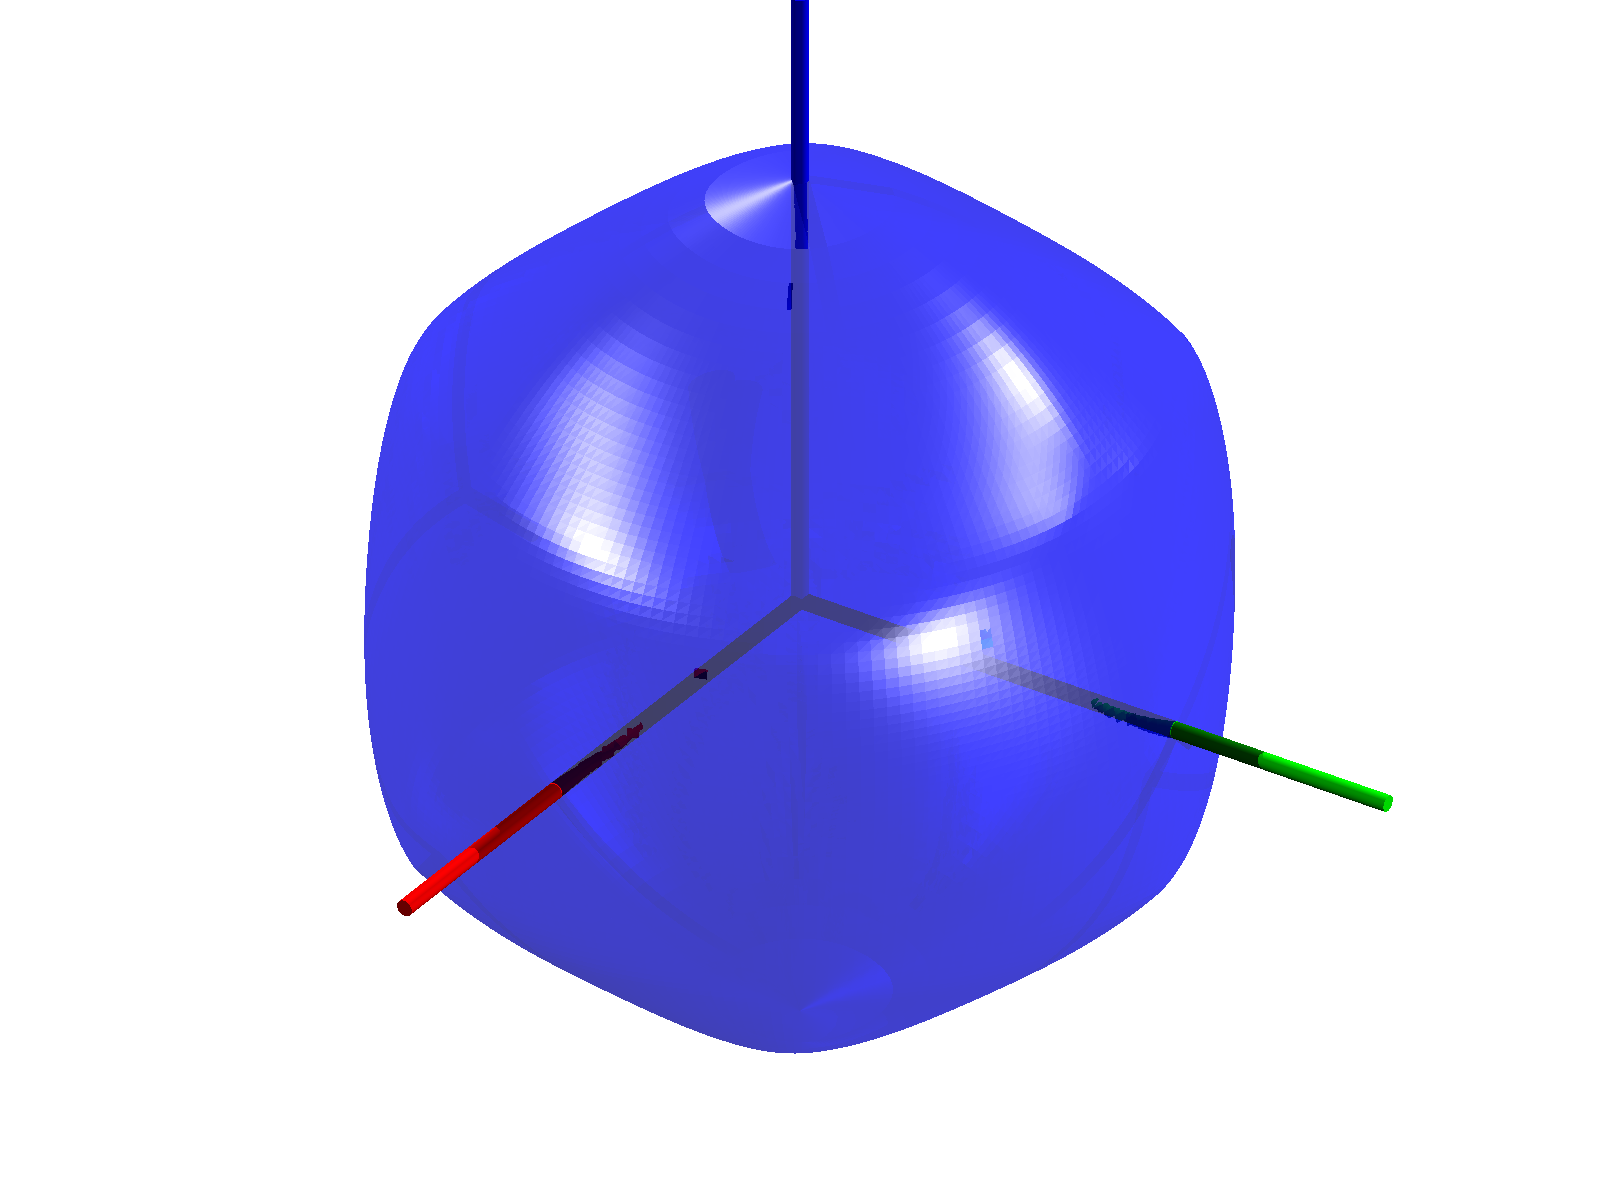
\includegraphics[width=4 cm]{slow_linbo3_1.png}
	\end{column}
	\begin{column}{4cm}
		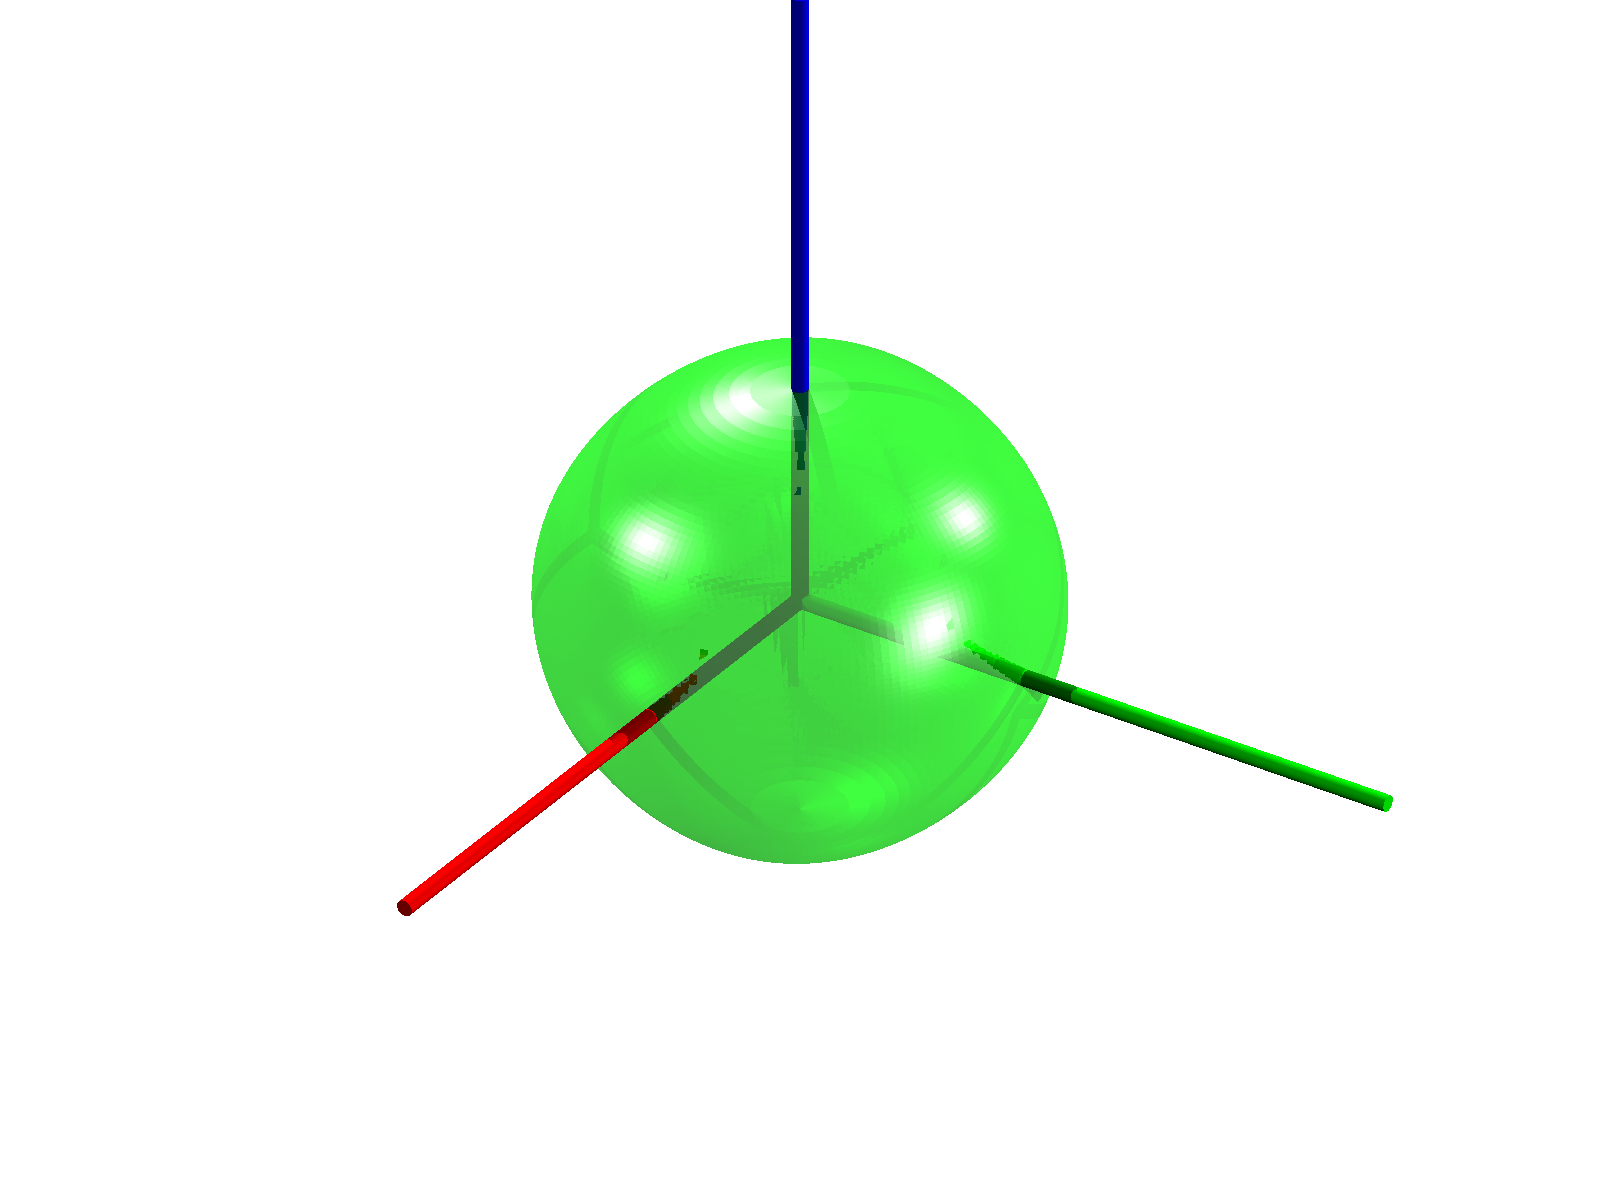
\includegraphics[width=4 cm]{slow_linbo3_2.png}
	\end{column}
\end{columns}
}

\subsection{Дифракция методом Фурье}
\frame{ 
  \frametitle{Дифракция на щели}
  
  Решение задачи о дифракции света на щели с использованием двумерного преобразования Фурье
  
  Дима
}
%

%Мобилограмма
% Tools:
% - C++ (С)
% - Qt (С)
% - mingw (С)
% - emacs (С)
% - git (С)
% - PovRay (П)
% Подбор констант:
% - кристоффель (Ю)
% - экстракция скоростей из файла (Ю)
% - градиентный спуск (П)
% - рой (Н)
% - отжиг (С)
% - дифракция (Д)

%\section{Подбор констант}
%\subsection{Метод отжига}\frame{}
%\subsection{Градиентный спуск}\frame{}
%\subsection{``Рой''}\frame{}

%\frame{
%\subsection{сПиСоК}
%\frame{\frametitle{unnumbered lists}
%\begin{itemize}
%\item Как выстрелить себе в ногу при помощи C++ и \LaTeX  
%\item *Курс для продвинутых
%\item Быдлокод
%\item BDD, TDD, Agile, XP и другие страшные слова
%\end{itemize} 
%}
%
%\frame{\frametitle{lists with pause}
%\begin{itemize}
%\item Introduction to  \LaTeX \pause 
%\item Course 2 \pause 
%\item Termpapers and presentations with \LaTeX \pause 
%\item Beamer class
%\end{itemize} 
%}
%
%\subsection{Lists II}
%\frame{\frametitle{numbered lists}
%\begin{enumerate}
%\item Introduction to  \LaTeX  
%\item Course 2 
%\item Termpapers and presentations with \LaTeX 
%\item Beamer class
%\end{enumerate}
%}
%\frame{\frametitle{numbered lists with pause}
%\begin{enumerate}
%\item Introduction to  \LaTeX \pause 
%\item Course 2 \pause 
%\item Termpapers and presentations with \LaTeX \pause 
%\item Beamer class
%\end{enumerate}
%}

%\section{Section no.3} 
%\subsection{Tables}
%\frame{\frametitle{Tables}
%\begin{tabular}{|c|c|c|}
%\hline
%\textbf{Date} & \textbf{Instructor} & \textbf{Title} \\
%\hline
%WS 04/05 & Sascha Frank & First steps with  \LaTeX  \\
%\hline
%SS 05 & Sascha Frank & \LaTeX \ Course serial \\
%\hline
%\end{tabular}}
%
%
%\frame{\frametitle{Tables with pause}
%\begin{tabular}{c c c}
%A & B & C \\ 
%\pause 
%1 & 2 & 3 \\  
%\pause 
%A & B & C \\ 
%\end{tabular} }
%
%
%\section{Section no. 4}
%\subsection{blocs}
%\frame{\frametitle{blocs}
%
%\begin{block}{title of the bloc}
%bloc text
%\end{block}
%
%\begin{exampleblock}{title of the bloc}
%bloc text
%\end{exampleblock}
%
%
%\begin{alertblock}{title of the bloc}
%bloc text
%\end{alertblock}
%}
\end{document}

